\documentclass[10pt,a4paper]{article}
\usepackage[utf8]{inputenc}
\usepackage[italian]{babel}
\usepackage{amsmath}
\usepackage{amsfonts}
\usepackage{amssymb}
\usepackage{graphicx}
\usepackage[left=2cm,right=2cm,top=2cm,bottom=2cm]{geometry}
\newcommand{\rem}[1]{[\emph{#1}]}

\author{Gruppo AC \\ Federico Belliardo, Francesco Mazzoncini, Giulia Franchi}
\title{Esercitazione N.3: Misure DC su transistor e NOT TTL.}
\begin{document}

\maketitle
\section{Scopo e strumentazione}
Verificare il funzionamento del transistor come amplificatore in un circuito in DC, determinando il guadagno in corrente continua ed analizzare l'uso del transistor in un circuito logico NOT.
\rem{Aggiungere strumentazione}

\section{Identificazione dei terminali dei componenti}

\paragraph{Misura della polarità delle giunzioni del diodo}
Per prima cosa abbiamo analizzando le polarità delle giunzioni del transistor,verificando che si trattasse effettivamente  di un diodo npn (abbiamo ottenuto valori positivi per le giunzioni BC e BE).

\rem{Tecnicamente questa cosa non è esplicitamente richiesta}
\paragraph{Misura delle resistenze del trimmer}
Utilizzando il multimetro digitale abbiamo misurato le resistenze del trimmer: ai suoi estremi la resistenza è risultata costante $R_{tot}= (102.7 \pm 0.8) k\Omega$, mentre la resistenza tra il terminale intermedio e uno dei due estremi è risultata variabile, prendenso l'uscita dalla parte delle scritte sul case la resistenza aumenta in senso orario

\paragraph{Controllo dello stabilizzatore di tensione}
Abbiamo montato il circuito in  figura \ref{circuito} verificando che  la $V_{out}$ rimanesse costante $V_{out} = (5.00 \pm 0.03) \, V$ (misurata con multimetro digitale) variando $V{in}$ da 6 a circa $20V$. 

\section{Misure in DC sul transistor}

misurando in precedenza le resistenze e il condensatore: $R_L = (0.977 \pm 0.008) \, k\Omega$ e $R_B= (46.7 \pm 0.4) \, k\Omega $ e $C=9.8 \pm 0.4) \, nF$
La tensione dell'alimentatore è stata misurata essere: $V_1 = (10.06 \pm 0.06) \, V$. 

\begin{figure}[!htb]
  \centering
  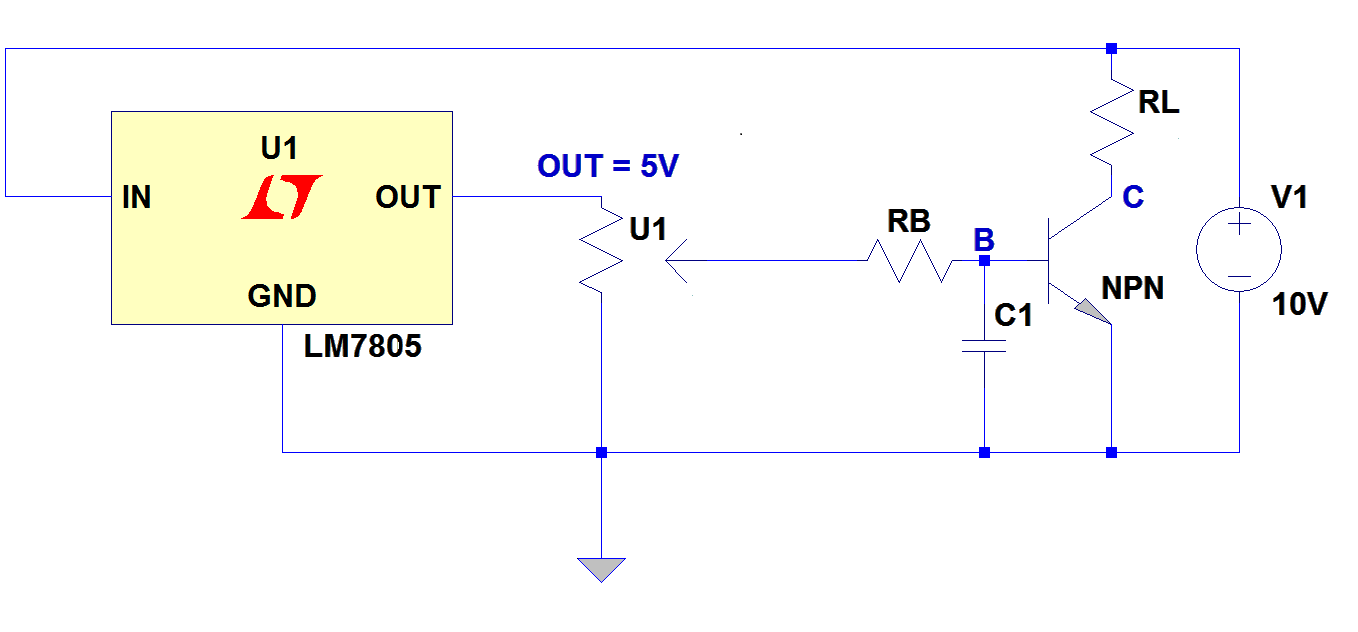
\includegraphics[scale=0.4]{circuito}
\caption{Circuito di amplificazione di correnti continue}
\label{circuito}
\end{figure}

\paragraph{Calcolo della retta di carico}
La retta di carico teorica è stata disgnata come retta tra due punti sul grafico delle curve cartteristiche del transistor: $I_C=\frac{V_1-V_{CE}}{R_L}$, come si vede nella figura
 \ref{caricoTeorica}.
 
\begin{figure}[!htb]
  \centering
  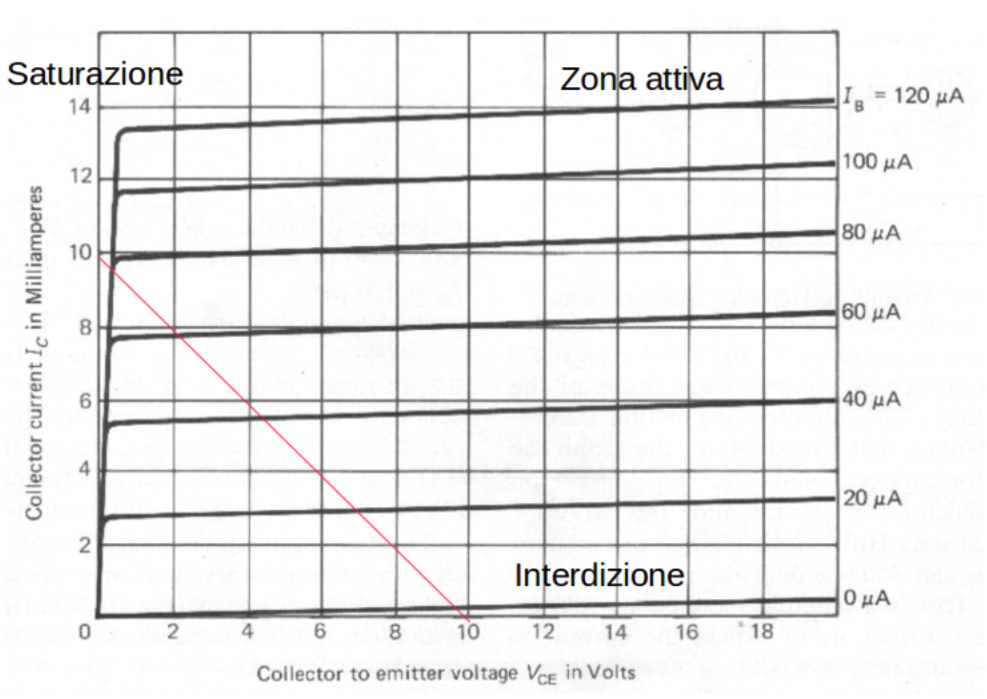
\includegraphics[scale=0.4]{rettaCarico.png} \label{caricoTeorica}
\caption{Circuito di amplificazione di correnti continue}
\label{circuito}
\end{figure}
 
\paragraph{Misure sul circuito}
Abbiamo collegato il multimetro digitale in parallelo alla resistenza $R_B$  e i due canali dell'oscilloscopio ai terminali B e C del transistor. In questo modo siamo stati in grado di misurare contemporaneamente la caduta di tensione $V_{R_B}$ ai capi della resristenza $R_B$, $V_{BE}$ e $V_{CE}$.
Abbiamo preso varie misure di $V_{R_B}$, $V_{BE}$ e $V_{CE}$  variando la resistenza del potenziometro (ruotando quindi la vite di regolazione). Grazie alle relazioni $I_B=V_{R_B}/R_B$ e $I_C=\frac{V_1-V_{CE}}{R_L}$ abbiamo potuto calcolare la corrente $I_B$ in ingresso alla base e la corrente del collettore $I_C$.
Il canale 1 è collegato alla base e il canale 2 è collegato al collettore.

Abbiamo riportato il tutto nella tabella \ref{misureDC}.

\begin{table}[!htb]\centering
\begin{tabular}{|c|c|c|c|c|c|}
\hline
4.16 & 0.02 & 0.32 & 0.01 & 0.88 & 0.03\\
3.97 & 0.02 & 0.3 & 0.01 & 0.86 & 0.03\\
3.22 & 0.02 & 0.31 & 0.01 & 0.84 & 0.03\\
2.92 & 0.02 & 0.31 & 0.02 & 0.86 & 0.03\\
0.0 & 0.0 & 10.0 & 0.3 & 0.08 & 0.0\\
3.26 & 0.02 & 0.2 & 0.007 & 0.74 & 0.02\\
2.88 & 0.02 & 0.24 & 0.008 & 0.74 & 0.02\\
2.55 & 0.02 & 0.216 & 0.007 & 0.74 & 0.02\\
2.36 & 0.02 & 0.228 & 0.007 & 0.74 & 0.02\\
2.06 & 0.01 & 0.26 & 0.008 & 0.74 & 0.02\\
1.49 & 0.01 & 2.24 & 0.07 & 0.72 & 0.02\\
1.34 & 0.01 & 3.0 & 0.1 & 0.7 & 0.02\\
1.13 & 0.01 & 4.2 & 0.1 & 0.7 & 0.02\\
0.963 & 0.005 & 5.0 & 0.2 & 0.68 & 0.02\\
0.744 & 0.004 & 6.2 & 0.2 & 0.66 & 0.02\\
0.545 & 0.003 & 7.3 & 0.2 & 0.64 & 0.02\\
0.406 & 0.002 & 8.2 & 0.3 & 0.64 & 0.02\\
0.229 & 0.002 & 9.0 & 0.3 & 0.64 & 0.02\\
0.0243 & 0.0002 & 10.0 & 0.3 & 0.5 & 0.02\\
0.0135 & 0.0001 & 10.0 & 0.3 & 0.296 & 0.009\\
0.0038 & 0.0001 & 10.0 & 0.3 & 0.084 & 0.003\\
0.0084 & 0.0001 & 10.0 & 0.3 & 0.184 & 0.006\\
0.0065 & 0.0001 & 10.0 & 0.3 & 0.14 & 0.005\\
0.0051 & 0.0001 & 10.0 & 0.3 & 0.112 & 0.004\\
\hline
\end{tabular}\\caption{Misure in Dc sul transistor} \label{misureDC}
\end{table} 

\begin{figure}[!htb]
  \centering
  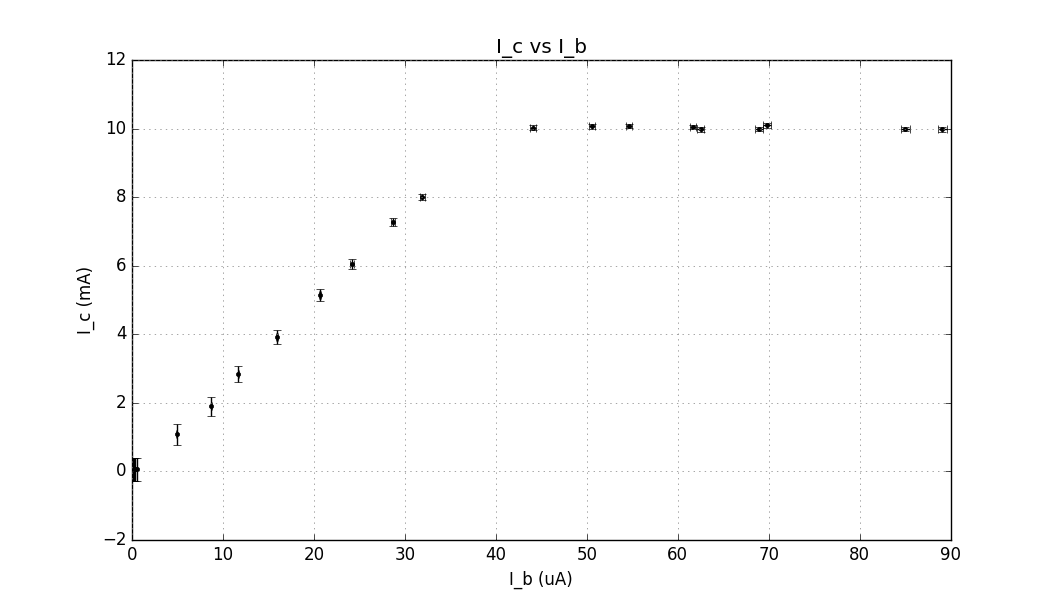
\includegraphics[scale=0.4]{IcIb.png} \label{IcIb}
\caption{Corrente di collettore vs. Corrente di base}
\label{circuito}
\end{figure}

\begin{figure}[!htb]
  \centering
  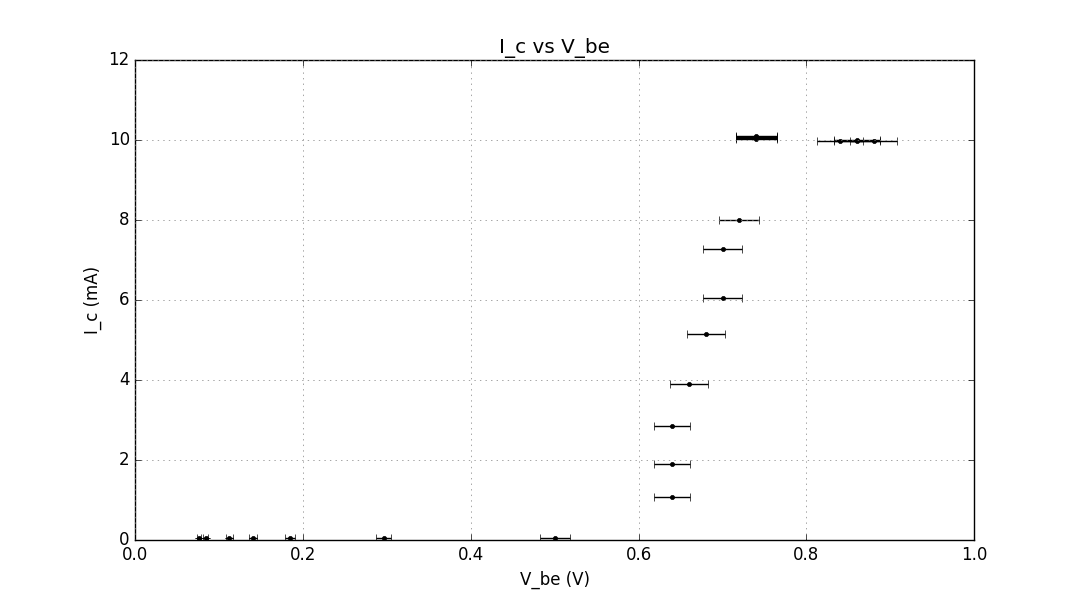
\includegraphics[scale=0.4]{IcVbe.png} \label{IcVbe}
\caption{Corrente di collettore vs. Tensione di base}
\label{circuito}
\end{figure}


\paragraph{Corrente di saturazione}
Abbiamo calcolato il guadagno del transistor  eseguendo un fit lineare di $I_C$ e $I_B$ con la  relazione $I_C=h_{FE}I_B+q$.
La massima corrente di collettore erogabile dal transistor è determinata dall'equazione di Kirchoff relativa alla maglia destra del circuito  $V_1 = R_L*I_C + V_{CE}$, quindi il massimo valore di $I_C$ si ha per il minimo valore di $V_{CE}$ ($V_sat$), che è una caratteristuca del transistor. Dalla corrente di saturazione che dipende 
  
%(array([ 0.2597147 , -0.21176614]), array([[  6.41851612e-05,  -1.31426841e-03],
%      [ -1.31426841e-03,   3.13037663e-02]]))
%Chisquare/ndof = 0.566115/6
%('p = ', 0.99693848309662825)

 
 \rem{Secondo me è più sensato misurare Ic e da questa dedurre la corrente di saturazione. La Ic si misura bene dai grafici la I di saturazione è piccola e non sono così convinto che si riesca a stimare bene dalla tabella}
 
\paragraph{Variazione della retta di carico al variare della tensione di alimentazione.}
 
Abbiamo ruotato la vite regolatrice del trimmer resistivo ottenendo $V_{CE}\simeq 5V$ per una tensione di alimentazione di $V_1 = 10 \, V$. Fissiamo questo valore della corrente $I_B$. Misuriamo  $V_{R_L}$ ai capi di $R_L$ con il multimetro digitale  e $V_{CE}$ tramite l'oscilloscopio al variare di $V_1$ tra $6 V$ e $16 V$. Tali dati sono riportati in tabella insieme a quelli di $I_C=V_{R_L}/R_L$.

%Questo ci permette di costruire una curva caratteristica del diodo a corrente di base costante. Questa può essere fittata da una legge esponenziale del tipo:
%$I_c = I_s e^{\frac{V_{BE}}{V_T}} (1-e^{-\frac{V_{CE}}{V_T}}$ quando il transistor è polarizzato in saturazione o in diretta è circa costante duqnue la curva da un andamento esponenziale che uò essere fittato. IL coeffiente che compare davanti alla curva esponenziale è esattamente il coefficiente hfe * I_b che è legato al valore asistotico dellla corrente I_c.
%Se queste approssimazioni fossero vere sempre allora la tensione di saturazione sarebbe nulla e la corrente di saturazione corrispondereebbe all'intercetta della retta di carico con l'asse delle ascisse.

Attraverso la misura della corrente di saturaturazione che estraiamo dal grafico $I_c - I_b$ possiamo fornire una stima della tensione di saturazione attraverso la legge delle maglie. Se valesse con esattattezza l'approssimazione enunciata sopra per correnti base arbitrariamente alte non potremmo avere tensioni di saturazione che sono un parametro fisico intrinseco della giunzione per cui l'approssimazione enunciata viene meno.

Per gli intervalli di tensione che possiamo utilizzare (per mantenere funzionante lo stabilizzatore) non misuriamo nessun dato nella zona di saturazione ma si osserva marcatamente l'effetto Early, come si vede in figura \ref{early}.


%Tensione di Early
%(array([  3.05190930e-05,   5.10298521e-03]), array([[  3.50480931e-12,  -2.12828657e-11],
%       [ -2.12828657e-11,   1.86911772e-10]]))
%('Early = ', -167.20631960490948)
%Chisquare/ndof = 7.413501/12
%('p = ', 0.82912270162218271) 

 
\section{Uso del transistor in un circuito logico NOT }
\paragraph{Montaggio del circuito}
Abbiamo montato il circuito rappresentato in  figura \ref{circuito2}.
\begin{figure}[!htb]
  \centering
 %TODO Aggiungere tutte le label su immagini e tabelle
  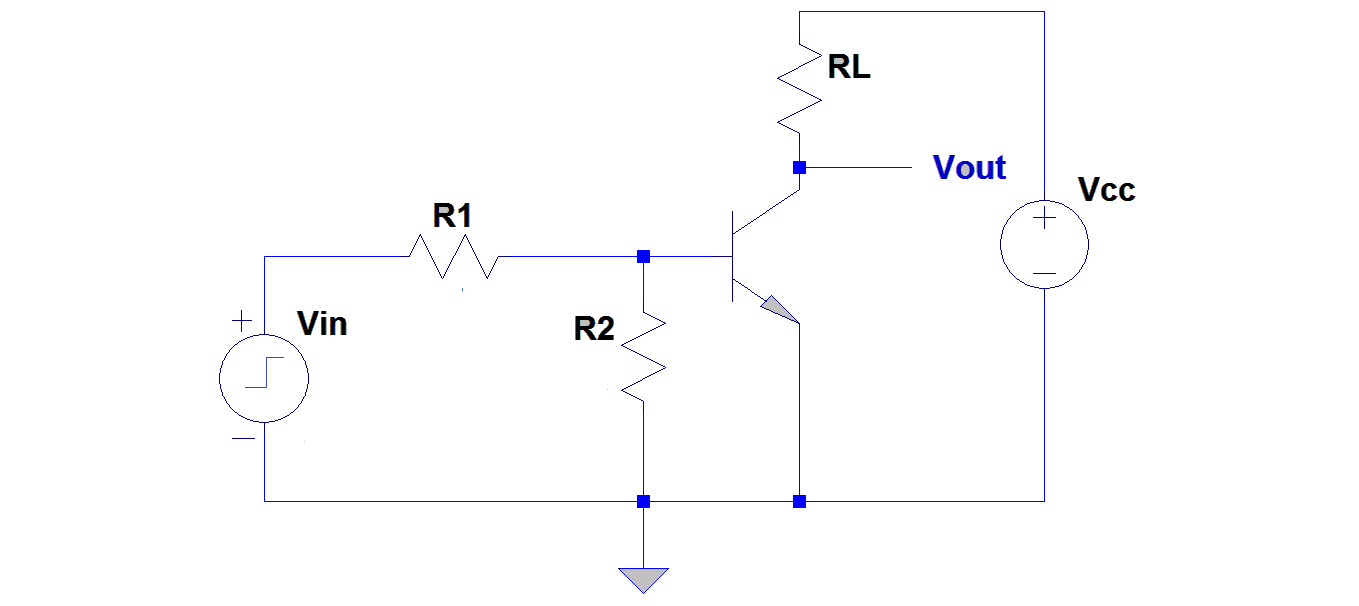
\includegraphics[scale=0.4]{circuito2} \label{circuito2}
\caption{Circuito logico NOT}
\label{circuito2}
\end{figure} 

In ingresso abbiamo collegato  il generatore di funzioni in modalità output pulse, il quale genera un’onda quadra oscillante tra $0 V$ e $5 V$. Abbiamo usato  il generatore di tensione $V_{CC}=$, con un valore scelto in modo tale da far funzionare il transistor  in regime di saturazione e di interdizione al variare di $V_{in}$. Le resistenze usate ( misurate con un multimetro digitale ) sono : $R_1=$ $R_2=$ $R_L=$


\paragraph{Verifica del corretto funzionamento del circuito}
\paragraph{Misura dei tempi di transizione di $V_{out}$ }

\paragraph{Discussione sui tempi di transizione di $ V_{out}$}

\rem{Non mi è chiaro perchè la capacità massima dovrebbe essere associata alla giunzione polarizzata diretta e non inversa dove la carica è maggiore, forse bisogna guardare la tensione}

\end{document} 